\chapter{The Consequences and Measurement of Inbreeding}
\label{cha:Lush_Chapter_21}
\index{Inbreeding|(}

Inbreeding is the mating of closely related animals. Everyone agrees
to that general definition, but there is much diversity of usage about
how closely related the mates must be before the mating should be
called inbreeding. Many practical breeders restrict the word inbreeding
to the mating of full brother and sister or of parent and offspring. Others
would call the mating of half brother and sister, or the mating of
grandparent to grandson or granddaughter inbreeding. The broad
scientific definition is that inbreeding is the mating of animals more
closely related to each other than the average relationship within the
population concerned. Such matings tend to make the offspring more
homozygous than if their parents were of average relationship to each
other. Mating of animals less closely related than the average of the
population concerned is outbreeding.

The population concerned would usually be the whole breed when
this definition is applied to animal breeding, but might be the race or
the whole species when considering the part which inbreeding may
play in evolution. The intensity of the inbreeding is very slight, however,
unless the mates are quite closely related or the inbreeding is continued
for many generations. This leads to the convenient situation
that the great majority of all breedings which take place within a pure
breed are practically neutral so far as any inbreeding or outbreeding
effect is concerned and may be classed as random breeding, even though
one does not know the average relationship within the breed. The practical
use of the definition that inbreeding is the mating of closely related
animals merely requires agreement as to how close that relationship
must be.

It is impossible to define inbreeding simply as the mating of related
animals. All animals that can be mated at all are related, at least slightly.
Each individual has two parents, four grandparents, eight great
grandparents, and so on, the number of ancestors doubling each generation.
In the tenth generation of its pedigree an animal will have more
than a thousand ancestors if there has been no inbreeding. If two ani-
thousand ancestors of the one cannot include any of the nearly contemporary
thousand ancestors of the other. If there has been no inbreeding,
each animal has more than a million ancestors in the twentieth generation
of its pedigree. If the pedigree is followed much further, these
numbers become greater than the number of animals alive at that time
could have been. For example, in man there are about three generations
to the century. The number of ancestors each person had living at the
time of William the Conqueror would be about $2{26}$, or roughly a little
more than 67 millions, if there had been no mating of relatives . Now
there never were that many people in Great Britain at any one time.
Anyone descended entirely from British ancestors must have had an
enormous amount of repetition of ancestors that far back in his pedigree,
especially since many individuals living at any one time leave no
descendants. One whose ancestors came from several nations has only
to follow his pedigree a few centuries further back (no further than to
900 A.D. at the outside) to find that, if there had been no mating of relatives,
he would have had more ancestors alive at that time than there
were people on earth!

This situation is more extreme in livestock breeding. The Brown
Swiss breed in the United States is descended entirely from 129 cows
and 21 bulls which were imported into this country. In American Rambouillet
pedigrees about 45 per cent of the lines traced back at random
end in sheep from the von Homeyer flock in Germany. Over half of
the random pedigree lines of the Shorthorn breed go to one bull,
Favourite. Similar things are true of other breeds, although few breeds
are yet explored in detail from this point of view. Moreover, this
includes only what has happened since pedigree recording began. That
is a comparatively short time --- about 150 years in the Shorthorns and
only about 50 years in the other two breeds mentioned.

The definition of inbreeding must be relative to some group or
population. Pure breeding, for instance, is inbreeding relative to the
whole species but need not be and rarely is inbreeding of noticeable
intensity relative to the breed. Figure~\ref{fig:Lush_Figure_34} illustrates
the situation diagrammatically from closest inbreeding to widest outbreeding. To the
left of random mating are the inbreeding matings while the outbreed ing
ones are to the right. The closeness of the two lines to each other in
Figure 34 represents how closely the mates are related to each other.
That ranges from complete identity in the case of self-fertilization (possible
in most plants but impossible in any farm animal) through close
relatives, members of the same breed, members of different breeds but
the same species, members of different species within the same genus,
and perhaps even members of different genera. The offspring of species
crosses usually exhibit some degree of sterility. Generic crosses are very
rare. Presumably the genotypes of the individuals are so unlike that
the union, even if possible at all, produces no living offspring.

\section*{THE CONSEQUENCES OF INBREEDING}
\index{Gene frequency|(}
\index{Heterozygosis|(}
\index{Homozygosis|(}

The primary effect of inbreeding is to increase the probability that
the offspring will inherit the same thing from sire and dam. This tends
to lower the percentage of heterozygosis in the population and to produce
relationships higher than 50 per cent. All the other effects of
inbreeding result from those. In each inbred line the genes which are to
be in the next generation are a sample of those which were in the preceding
generation. Because the sample is small the gene frequency in it
will often by chance differ considerably from the gene frequency in the
generation from which the sample came. Thus the gene frequency can
wander back and forth until it reaches either zero or one. Then the line
is homozygous for that particular gene or its allel. This homozygosis
cannot be lost, except by mutation, as long as the inbreeding is continued.
The genes which are heterozygous are still subject to the
possibility of becoming homozygous each generation the inbreeding
continues. The fewer animals there are in the inbred line the smaller
is the sample of gametes which are needed to constitute the next generation
and the farther the frequency of each gene can drift up or down
in any one generation.

\begin{figure}
	\centering
    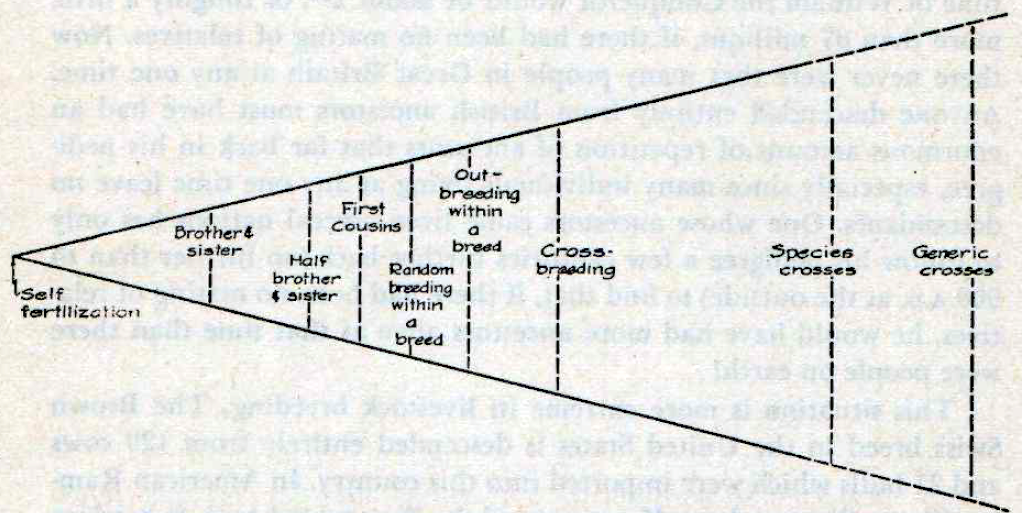
\includegraphics[width=\textwidth]{Figure_34.png}
    \caption{Degrees of inbreeding arranged according to the relationship between mates.}
    \label{fig:Lush_Figure_34}
\end{figure}

Because this change in gene frequency is random (equally likely to
be up or down), inbreeding is in conflict with selection whenever selection
is tending to keep a gene at some equilibrium frequency, as when
the heterozygote\index{Selection!for heterozygotes|(} is preferred. Inbreeding is continually causing the
gene `frequency to drift away from that equilibrium point in either
direction and selection is continually tending to take it back there.
When the inbreeding is very mild and selection is intense, the gene frequency
cannot get far from its equilibrium value. But when the
inbreeding is intense it may overwhelm selection and carry gene frequencies
far away from their equilibrium values, some above and some
below.

If the inbreeding is intense and continues long enough, and if there
are no mutations, the ultimate condition approached in each inbred
line is complete homozygosis in all pairs of genes. In some pairs it will
be the less desirable and in other pairs the more desirable gene which
becomes homozygous. Each inbred line is likely to differ from every other
inbred line in regard to which particular combination of genes
becomes homozygous in it, if many different pairs of genes are involved.
Inbreeding in animals almost never comes close to complete homozygosis
in actual practice. Even self-fertilized plants reach an equilibrium
point where the further loss of the remaining small amount of heterozygosis
just equals the new heterozygosis which mutations produce in
each generation. Mutations\index{Mutations} are so rare that for practical purposes they
can be neglected in considering inbreeding but they are mentioned
here for completeness.

The Mendelian basis of the inbreeding effect can be illustrated most
simply by the extreme case of self-fertilization. Each generation in each
inbred line consists of one individual in which, of course, each gene is
either homozygous or heterozygous. That is, gene frequency can have
only the values: .0, .5, or 1.0. Genes which are already homozygous in
the whole line must remain so as long as the inbreeding continues,
unless a mutation occurs. Pairs of genes which are heterozygous may be
considered as a population of the two kinds of genes in equal numbers,
from which two genes are to constitute the population in the next generation.
The probabilities that those two will be \textit{AA}, \textit{Aa}, or \textit{aa}, are in
the ratio 1 : 2 : 1. Thus half of all heterozygous genes in a self-fertilized
individual may be expected to become homozygous in its offspring.
Selection favoring either homozygote will tend to hasten the rate of
approach to homozygosis, while selection favoring the heterozygote will
tend to retard it. If there are many heterozygous pairs of genes, several
will become homozygous in every individual; and selection can have
only trivial effects in delaying any such rapid rate of approach toward
homozygosis. For example, if a self-fertilized individual is heterozygous
for 10 pairs of genes, only 1 offspring in 1,024 would be as heterozygous
as its parent. Even in species with reproductive rates which would permit
intense selection, it would be impossible to recognize genotypes
accurately enough to find such a rare heterozygous offspring every time
without mistake. If the inbreeding rate were lower or the number of
heterozygous genes were less, selection would have more chance to alter
the consequences of inbreeding. Actually, with each animal heterozygous
for scores of genes, many of which have only minor effects which
may be blurred by the effects of environment, the difference between
intense selection and no selection under self-fertilization has little more
effect on the outcome than the fate of a man dropped into the Niagara
River just a few yards above the falls would be affected by whether he is
a good swimmer or a poor swimmer! The difference in swimming ability
might be of tremendous importance if he were in comparatively
still water, as is roughly analogous to the situation in a population in
which the inbreeding is very mild, but would only rarely make a detectable
difference in the results in the presence of the much more powerful
force of the swiftly moving water.
\noclub[3]
\index{Selection!for heterozygotes|)}

Self-fertilization is impossible in the higher animals, but the Mendelian
basis of the inbreeding effect may be illustrated with the continued
inbreeding of full brother and sister. For each allelic set of genes
this constitutes a population of four genes-two in the sire and two in
the dam-from which four are to come to constitute the next generation.
Gene frequency can have only the values: .00, .25, .50, .75, or 1.00.
Although only one of them will occur in any one generation in any one
line, six different types of matings are possible. Those types are:

\begin{table}[h]
	\centering
	\begin{tabular}{C{3cm}C{3cm}C{3cm}}
						&						& Frequency of \textit{A} in \\
		Type 			& Mating				& this inbred line \\
		1				& \(AA \times AA\)		& 1.00 \\
		2				& \(AA \times Aa\)		& .75 \\
		3				& \(AA \times aa\)		& .50 \\
		4				& \(Aa \times Aa\)		& .50 \\
		5				& \(Aa \times aa\)		& .25 \\
		6				& \(aa \times aa\)		& .00 \\
	\end{tabular}
\end{table}

\noindent
If either the first or the last of these prevails, that line will remain
homozygous for that gene indefinitely, unless a mutation occurs. If
either the second or the fifth type prevails in one generation, there is
one chance in four that this line will become homozygous in the next
generation, two chances in four that it will remain the same, and one
chance in four that the next generation will be like the fourth type of
mating. When the line is of the third type, it will change to the fourth
type in the next generation. When it is of the fourth type, there is one
chance in eight that it will become homozygous in the next generation,
four chances in eight that it will change to types two or five, one chance
in eight that it will change to type three, and two chances in eight that
it will remain the same. Once the inbred line becomes type one or type
six, it remains that way. It can shift back and forth among the other
four types; but from them it will occasionally drift into types one or six,
from which it cannot return. Hence the ultimate end of all such lines
would be type one or type six if the inbreeding were continued long
enough. The drift from one type to another is so rapid in a population
as small as a line inbred full brother by sister that, after the inbreeding
gets well ·under way, nearly one-fifth of all the genes which are still heterozygous
in the line at any given time become homozygous in the next
generation. In larger populations the gene frequency would fluctuate
less extremely, but in any finite population it would do some shifting.
Inbreeding is only an extreme form of a process which exists to some
degree in all populations. The fact that the number of breeding individuals
in the poplation is finite permits gene frequency to vary
because of the sampling which takes place when the genes of one generation
are replaced by the genes of the next.

This Mendelian proof of the nature of the inbreeding process was
studied as long ago as 1914 by Fish, Jennings, and
Pearl,\footnote{\textit{Amer. Nat.}, 48:57--62, 491--94, 693--96, and 759--61.}
but it becomes extraordinarily difficult to follow even for regular
inbreeding systems milder than full brother by sister and practically
impossible to follow in the irregular inbreeding which occurs with farm
livestock. Wright in 1921 published a generalized explanation of the
consequences of milder forms of regular inbreeding and of irregular
inbreeding. In 1931 he generalized this still further to establish the
identity of the inbreeding effect and the general consequences of finite
population size, even in cases which we would not ordinarily call
inbreeding.\footnote{\textit{Genetics}, 6:124--43 and 16:106--29.}
\noclub

By changing heterozygotes to homozygotes, inbreeding brings to
light many of the recessive genes which would otherwise remain hid den.
Most recessive genes have less desirable effects than their alleles.
Inbreeding, therefore, usually lowers the average outward merit of the
inbred animals. Inbreeding permits more rapid improvement of the
breed by getting the recessive genes out from the shelter of their dominant
alleles so that they can be found more readily. For example, if 1
per cent of the calves in the Aberdeen-Angus breed are now born red
and the breeders were all to begin suddenly to inbreed as intensely as
mating parent and offspring or full brother and sister, the percentage of
red calves would in the first generation of inbred calves go up more
than threefold. The distribution of the genotypes\index{Zygotic ratios} before and after the
inbreeding would be as follows:

\begin{table}[h]
	\centering
	\begin{tabular}{L{6cm}L{2cm}L{2cm}L{2cm}}
		Before inbreeding:					& 81 \% \textit{BB}					& 18 \% \textit{Bb}	& 1    \% \textit{bb} \\
		After one generation of inbreeding:	& 83\nicefrac{1}{4}\% \textit{BB}	& 13 \nicefrac{1}{2}\% \textit{Bb}	& 3 \nicefrac{1}{4}\% \textit{bb}
	\end{tabular}
\end{table}

\noindent
The percentage of heterozygosis would decrease one-fourth, the genes
which would have been in heterozygous individuals now being equally
divided among the two kinds of homozygotes. The gene frequency has
not changed, but only the zygotic ratio. On account of dominance, the
desirable increase in \textit{BB} and decrease in \textit{Bb} individuals would not be
apparent outwardly. The only readily apparent change would be the
threefold increase in the proportion of red calves.
\index{Gene frequency|)}

For ages men have observed this general fact that inbreeding tends
to produce a certain amount of degeneration or decline in individual
merit. Formerly it was thought that the inbreeding in some mysterious
way actually damaged the inheritance and thus directly caused this
degeneration. Now it is understood that the inbreeding merely acts
somewhat as a detective does in uncovering crime -- not in creating it.
The undesired recessive genes are there all the time, but homozygous
recessive individuals appear more frequently when inbreeding begins.

More than any other breeding method, inbreeding tends quickly to
separate the population into many distinct families, each of which is
uniform within itself but distinct from others. This splitting of the
population into distinct families offers more opportunity for selection
between families than could take place in a random-bred population.
Inbreeding without selection leads toward a variable\index{Variation!increased by inbreeding} population composed
of unlike lines. If inbreeding were carried to completeness without
selection, the composition of the resulting population would be the
same as if the gametes from the initial population had suddenly been
transformed into zygotes by doubling all their chromosomes. If all the
genes acted only in an additive way, the genetic variance in the new
entirely homozygous population would be exactly twice what it was in
the original random-bred population, but would be entirely between
families, with no genetic variance within families. If many of the lines
were discarded, the population as a whole might then become more
uniform than it was before the inbreeding began; but that would be
primarily the result of discarding the poorer inbred lines rather than
a result of the inbreeding itself.

Inbreeding is especially powerful in forming \index{Family differences|(}families because the
genetic likeness of the mates does not depend upon the breeder's ability
to recognize which animals have similar genes when he mates them
together, as is the case with selection and with assortive mating. The
effects of inbreeding are not limited by the breeder's mistaking the
effects of environment, dominance, or \index{Epistatic effects}epistasis
for the effects of genes,
as the effects of those other breeding methods are. That is why inbreeding
is particularly powerful and useful in breeding for characteristics
which are only slightly hereditary. This difference also leads to the general
situation that under an inbreeding system the mates are more alike
in their heredity than they are in their appearance, whereas under
assortive mating they appear more like each other than they really are.
Where the correlation between genotype and phenotype is low, this
difference may be extreme.

Inbreeding may also produce some degeneration of individuals by
scattering the genes which in certain combinations produce a desirable
effect but which separately produce neutral or undesirable effects. If
there really is much of this epistasis, and if a breed has been under strict
selection for some time, there will have been a tendency to bring together,
in combinations where they will show good effects, those genes which
nick together well. Since most of those combinations will still be heterozygous,
at least for some of the genes concerned, any inbreeding will
tend to separate those combinations again and thus will lead to some
apparent loss of individual merit in addition to that coming entirely
from uncovering recessives.

Also inbreeding will lower the average merit of the population
directly by reducing heterozygosis among those pairs of genes in which
the heterozygote is more desirable than either homozygote.
\index{Family differences|)}

\section*{MEASURING THE INTENSITY OF INBREEDING}
\index{Inbreeding!measurement of|(}

Since the primary effect of inbreeding is to increase the probability
of receiving duplicate genes from sire and from dam, the measure of
inbreeding ought to be one which shows how much decrease in heterozygosis
is to be expected from that particular kind of inbreeding. Such
a coefficient will mean little so far as concerns one pair of genes in one
animal, but it may tell much about the average condition of one pair of
genes in a whole herd or breed, and it will tell much about the average
heterozygosity of the whole group of genes in an individual animal.

There seems to be no possibility that we shall ever be able to count
the actual number of heterozygous genes in each animal. Each animal
must be compared with the average condition in the population chosen
for a base. The most convenient population to use for a base in animal
breeding is usually the breed at the date to which the pedigrees are
traced. It is then assumed that those foundation ancestors were a random
sample of the breed at that date. Occasionally that assumption
may lead to some error, when a pedigree if traced another generation or
two would have revealed that the foundation ancestors were highly
related to each other.

The inbreeding coefficient (devised by Wright\footnote{\textit{Amer. Nat.},
56:330--38 or \textit{Jour. Heredity}, 14:339--48. A different measure of
inbreeding had been proposed earlier by Pearl (\textit{Amer. Nat.},
48:513--23, 1914). It was based on a ratio between the number of different
ancestors an animal actually had and the number it would have had if there
had been no inbreeding. In general, it was a useful standard for comparing
different intensities of inbreeding but in many cases gave inconsistent
results. It is now of historical interest only, although references
to it occasionally are made in current writings.}) starts at zero for
random mating, in which case the probable proportion of heterozygosis
is $2q (1 - q)$, and increases toward 100 per cent as the probable proportion
of heterozygosis goes toward zero. The inbreeding coefficient has
to be expressed relatively rather than in terms of the actual number of
heterozygous genes. For example, if the average Shorthorn of 1910 was
heterozygous for 200 pairs of genes, then a Shorthorn, so bred that its
inbreeding coefficient is 25 per cent relative to 1910 as a base date, will
probably be heterozygous for only 150 pairs of genes. On the other
hand, if the average Shorthorn in 1910 was heterozygous for a thousand
pairs of genes, a Shorthorn showing an inbreeding coefficient of 25 per
cent would probably still be heterozygous for about 750 pairs. An
inbreeding coefficient of 25 per cent in one breed may not mean the
same number of heterozygous genes as an inbreeding coefficient of 25
per cent in another breed. This need not bother us, since we really
take that into account at the start when we recognize that the one breed
is more uniform than the other.

The inbreeding coefficient of an individual is exactly one-half the
relationship between its parents unless those parents are themselves
inbred, in which case some correction (usually small) for that is to be
made. The formula is as follows:

\[ F_X = 1/2 \Sigma [(1/2)^n(1 + F_A)] \]

\noindent
where $F_X$ is the inbreeding coefficient of animal X; \textit{n} is the number of
generations (the intervening segregations) in a line by which sire and
dam are related; $F_A$ is the inbreeding coefficient of the common ancestor
($A$) out of whom that line of descent divides; and $\Sigma$ is the summation
sign meaning that each such path of relation between sire and dam is to
be evaluated separately and then all the results are to be added together.
The $\Sigma [(1/2)^n]$ part is exactly the formula discussed in the preceding
chapter for relationship when no inbreeding is involved. Thus, when
the parents are not inbred the inbreeding of the offspring is exactly
half of the relationship of its parents to each other. The factor $(1 + F_A)$
corrects for the fact that, because an inbred ancestor (\textit{A}) is probably
homozygous for \index{Genes, number of}more pairs of genes than a random-bred ancestor, two
gametes coming out of it will usually be alike in more of their genes
than two gametes from a non-inbred ancestor. As a numerical example, if a
non-inbred ancestor is heterozygous for 200 pairs of genes, the average
situation concerning two gametes from it is that they will have
unlike genes in about 100 of those loci. From the same population an
ancestor inbred 25 per cent would probably be heterozygous for only
about 150 pairs of genes. Two gametes from it would be unlike in only
about 75 loci. If the ancestor were complete inbred (\(F_A = 1.0\)), which
can only be approached but not actually reached in farm animals), all
the gametes from it would be exactly alike. This would be equivalent
to eliminating one Mendelian segregation, and hence one 50 : 50 chance
of unlikeness, from each line of relationship between sire and dam
through this ancestor.

\index{Sampling nature of inheritance|(}
As a Mendelian example of why the formula for the inbreeding
coefficient takes the form it does, consider the case of \textit{X}, a
double grandson of \textit{A}, with pedigree as follows:

\begin{figure}[h]
	\centering
    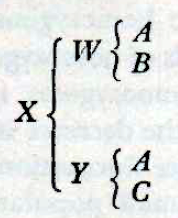
\includegraphics[width=0.3\textwidth]{Page_273.png}
    \label{fig:Lush_Figure_Page-273}
\end{figure}

\noindent
\textit{W} and \textit{Y} are related to each other 25 per cent, and
\(F_X = 12.5\) per cent or \nicefrac{1}{8}. The one line of descent connecting
\textit{W} and \textit{Y} is \(W \leftarrow A \rightarrow Y\). To
see what will probably happen to the genetic composition of \textit{X}, we will
consider a pair of genes, \textit{Rr}, for which \textit{A} is heterozygous.
What is the probability that \textit{X} is homozygous (\textit{RR} or
\textit{rr}) through having received duplicate genes in this locus from
\textit{A}? We are not interested in genes
from \textit{B} or \textit{C} since, as far as the pedigree shows, they are unrelated to
each other or to \textit{A}, and our inbreeding coefficient measures only how
many of the genes heterozygous in the foundation animals (those at the
base date to which the inbreeding was computed) have probably
become homozygous in \textit{X} because of its inbreeding. \textit{W} and \textit{Y} are each
equally likely to have received \textit{R} or \textit{r}. They each are equally likely to
transmit whichever gene (\textit{R} or \textit{r}) they did receive from \textit{A}, or the allel to
it which each received from its other parent. The probabilities with
respect to the genes of the \textit{Rr} pair in \textit{X} are as follows:
\begin{align*}
 ~&\text{4 chances in 16 that neither gene came from } A\text{.} \\
 ~&\text{4 chances in 16 that } R \text{ came from } A \text{ but the other allel came from a
grandam.} \\
 ~&\text{4 chances in 16 that } r \text{ came from } A \text{ but the other allel came from a
grandam.} \\
 ~&\text{2 chances in 16 that both genes came from } A \text{ and } X \text{ is } Rr\text{.} \\
 ~&\text{1 chance in 16 that both genes came from } A \text{ and } X \text{ is } rr\text{.} \\
 ~&\text{1 chance in 16 that both genes came from } A \text{ and } X \text{ is } RR\text{.}
\end{align*}

\noindent
If either of the last two events happened, \textit{X} is homozygous for a gene
for which \textit{A} was heterozygous. Together the last two events have a
probability of one-eighth of happening. When we say that the inbreeding
coefficient of \textit{X} is \nicefrac{1}{8}, we are saying that \textit{X} is probably homozygous
for \nicefrac{1}{8} of the genes which were heterozygous in the ancestors at the
foundation or base date to which the pedigree of \textit{X} was traced. If we
combine the probabilities of each of the above events happening, and
include also what would have happened if \textit{A} had been \textit{RR} or \textit{rr}, we
find that if many are bred like \textit{X} (i.e., with the inbreeding
that results from being double grandsons) from a population of grandparents
whose zygotic frequencies\index{Zygotic ratios} are: $q^{2}RR : 2q(1 - q)Rr : (1-q)^{2}rr$,
then the most probable zygotic ratio among those bred like \textit{X} is:
$[q^2 + Fq(1 - q)]RR : 2q(1 - q)(1 - F)Rr: [(1 - q)^{2}+Fq(1 - q)]rr$.
In other words this amount of inbreeding will probably transform \nicefrac{1}{8}
of the heterozygous gene pairs into homozygous ones, half of that \nicefrac{1}{8}
being added to each of the two kinds of homozygotes. Thus the inbreeding
is impartial between the two homozygotes, tending on the average
to add to each of them one-half of the decrease it causes in the frequency
of heterozygotes. Of course chance fluctuations concerning that fraction
are large in the necessarily small population which is any one
inbred line.
\index{Sampling nature of inheritance|)}

The measurement of inbreeding, even in the most complicated pedigrees,
is simply computing the amount of heterozygosis probably lost
because of the inbreeding. In the simpler cases, where sire and dam are
related through only one or two lines, the computations are easy. It is
only necessary to find the common ancestor, count and add the number
of segregations between sire and ancestor and between dam and ancestor
and compute \nicefrac{1}{2} to one higher power than that. If much of this is to
be done, it is convenient to memorize or have handy a table of (\nicefrac{1}{2})$^n$ for
values of \textit{n} from 1 to 7 or 9. When \textit{n} is more than 6, this fraction is less
than 1 per cent. Little is gained by investigating any one relationship
too distant to contribute even this much, although if there are very
many such lines, their total might be important.

In the more complicated cases it may be necessary and is convenient
to draw the pedigrees in the arrow style shown in the middle and bottom
of Figure~\ref{fig:Lush_Figure_35}. In this form of pedigree each ancestor is shown only
once. An arrow leads from it to each descendant. Unless it had more
than one descendant it did not provide any inbreeding itself, but merely
transmitted to its one offspring some of the genes received from its
parents. When pedigrees are drawn in arrow style it is usually easy to
see at a glance what kind of a breeding system had been used and
toward which ancestors the inbreeding had been directed. Printing
difficulties are an obstacle to using the arrow style widely, as well as the
fact that in most pedigrees in sale catalogues and advertisements there is
little or no inbreeding visible, and in many cases the owner does not
wish to call attention to that small amount. At the bottom of Figure~\ref{fig:Lush_Figure_35}
are shown the computations for the amount of inbreeding coming from
each line through which sire and dam are related.

\begin{figure}
	\centering
    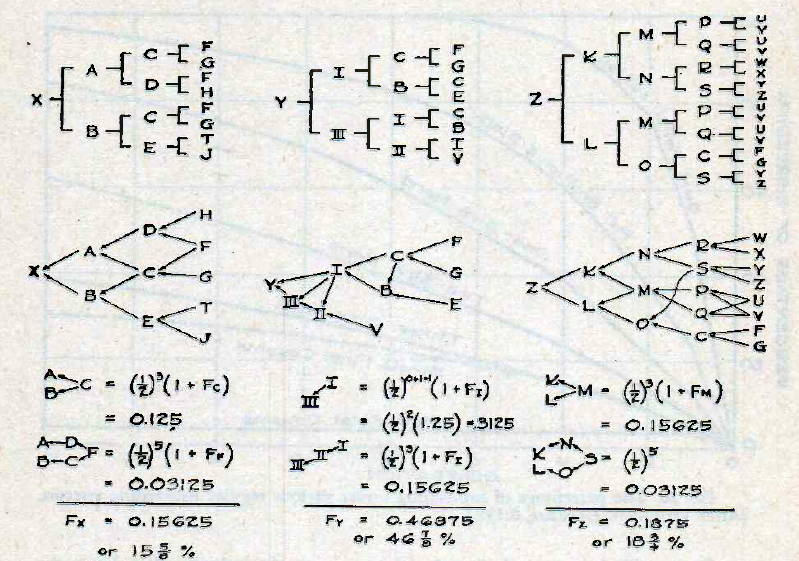
\includegraphics[width=\textwidth]{Figure_35.png}
    \caption{Three pedigrees illustrating how the coefficient of inbreeding is computed.}
    \label{fig:Lush_Figure_35}
\end{figure}

In pedigrees from experiments where inbreeding has been conducted
for many generations, the computations may become very intricate.
Occasionally that happens in purebreeding where, as in the case of
the ``straightbred'' Anxiety 4th Herefords, a family has been bred with
little or no outside blood for more than five or six generations. For
practical purposes it is usually sufficient in such cases to compute the
inbreeding for only the last four or five generations and assume that the
ancestors at that date were typical of this family, thus making the coefficient
relative to this family at that date instead of making it relative to
the whole breed.

Figure~\ref{fig:Lush_Figure_36} shows for some regular inbreeding systems the sharp differences
between the most intense systems theoretically possible and
some of the milder ones which might more readily be practiced with
farm animals. The milder inbreeding systems are much less intense at
the start but if continued long enough in an entirely closed population
can bring the population to a high degree of homozygosis. How very
long that would be in terms of one breeder's lifetime can be seen by
multiplying the number of generations in Figure~\ref{fig:Lush_Figure_36} by two and one-half
years in the case of swine, four or five years in the case of cattle and
sheep, and ten or more years in the case of horses.

\begin{figure}
	\centering
    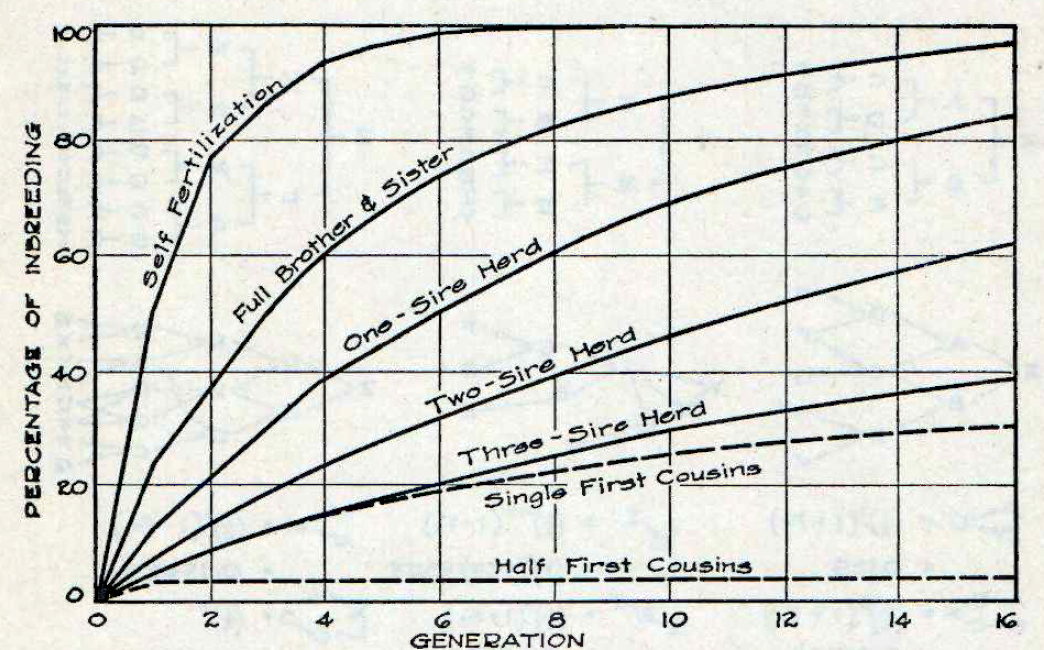
\includegraphics[width=\textwidth]{Figure_36.png}
    \caption{The percentage of inbreeding under various regular inbreeding systems.
(After Wright in Genetics, 6:172.)}
    \label{fig:Lush_Figure_36}
\end{figure}

Figure~\ref{fig:Lush_Figure_37} shows similarly what happens to the relationship between
full brothers under the same inbreeding systems. Unrelated families
are apt to drift farther apart under inbreeding than they would under
random mating, but each tends to become uniform within itself. A one-sire
herd where no females are ever purchased but each new sire is
unrelated to the herd will approach but never rise above the level of an
average relationship of 33\nicefrac{1}{3} per cent between herd mates. By contrast
a one-sire herd in which neither sires nor dams are purchased and there
is no overlapping of generations will even in the first inbred generation
reach an average relationship of 39 per cent between herd mates and in
the next generation will pass 50 per cent. The whole herd will then be
more uniform than if all members were full sibs.
\index{Inbreeding!measurement of|)}

\begin{figure}
	\centering
    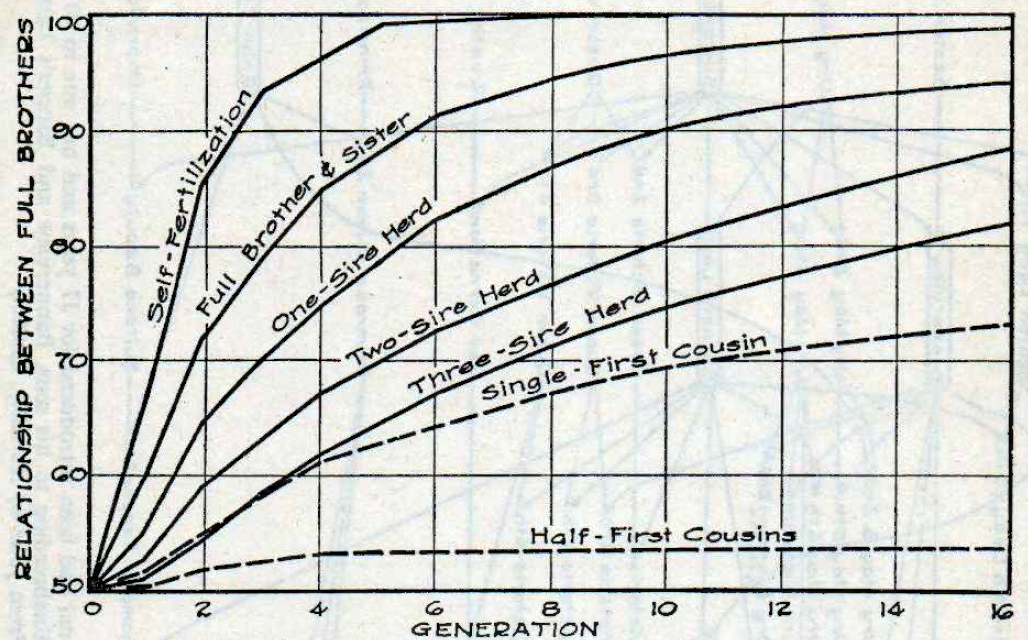
\includegraphics[width=\textwidth]{Figure_37.png}
    \caption{The relationship between full brothers under various regular inbreeding
systems. (After Wright in \textit{Genetics}, 6:170.)}
    \label{fig:Lush_Figure_37}
\end{figure}

\section*{THE RATE OF INBREEDING IN ISOLATED POPULATIONS}
\index{Inbreeding!in isolated populations|(}

The complete formula for the inbreeding coefficient is unwieldy in
estimating the consequences of any breeding plan which is to extend for
more than a few generations. For example, one might have a herd of
cattle just big enough to justify keeping two sires at a time; and he
might plan to raise his own sires without ever introducing any new
stock from other herds. Soon his sires would be related to all the females
on which they were to be used, but this relationship would vary. Many
would be half sisters, some would be cousins, some would be less closely
related older cows from the preceding generations, a few might be full
sisters, dams, three-quarter sisters, etc. Figure~\ref{fig:Lush_Figure_38}
shows an actual exam ple of this from a Shorthorn herd where only one sire
and no females 	had been bought in 20 years.\footnote{\textit{Jour. of Heredity},
25:208--16.} To compute the average inbreeding in
such an actual herd after it has been produced is a tedious job and not
very practical, since the animals are already produced whether one
likes them or not. For practical purposes one wants to estimate and
compare the consequences of various possible plans, so that the one
thought most favorable can be adopted and the less favorable ones left
untried.

If a population is kept entirely closed to outside blood, about
\(\dfrac{1}{8M} + \dfrac{1}{8L}\) of the remaining heterozygosis will
be lost per generation, where \textit{M} is the number of males and
\textit{L} is the number of females reaching breeding age in each
generation.\footnote{For the derivation of this formula see: \textit{Genetics},
16: 107--11. Strictly speaking, \textit{M}
and \textit{L} are the ``effective numbers.'' They would equal the actual census numbers in
the simple case in which all males and all females had equal chance to leave offspring.
Many conditions can cause the effective numbers to be smaller than the actual
numbers. At least a few of these will occur in practice. Hence the formula will
underestimate the amount of inbreeding in closed populations. See \textit{Amer. Nat.}, 74:241--47. 1940.} In a herd where there are 2 sires
and 40 females in active use, this would be \nicefrac{1}{16} + \nicefrac{1}{320}, or about 6.6
per cent of the remaining heterozygosis. In animal breeding, \textit{L} will
usually be so much larger than \textit{M} that the term $\dfrac{1}{8L}$ can be neglected
without much error. Then the formula becomes simply $\dfrac{1}{8M}$ giving
inbreeding rates of 12 per cent, 6 per cent, 4 per cent, and 3 per cent per
generation, respectively, for one-sire herds, two-sire herds, three-sire
herds, and four-sire herds, closed to all outside blood. These rates can
be reduced somewhat by avoiding inbreeding as far as possible under
those conditions. No reduction at all could be produced in a one-sire
herd, only a small reduction in a two-sire herd, more in a three-sire
herd, etc. The maximum effect of avoiding all inbreeding as far as possible
within a closed population tends toward halving the rate given by
the formula.

\begin{figure}
	\centering
    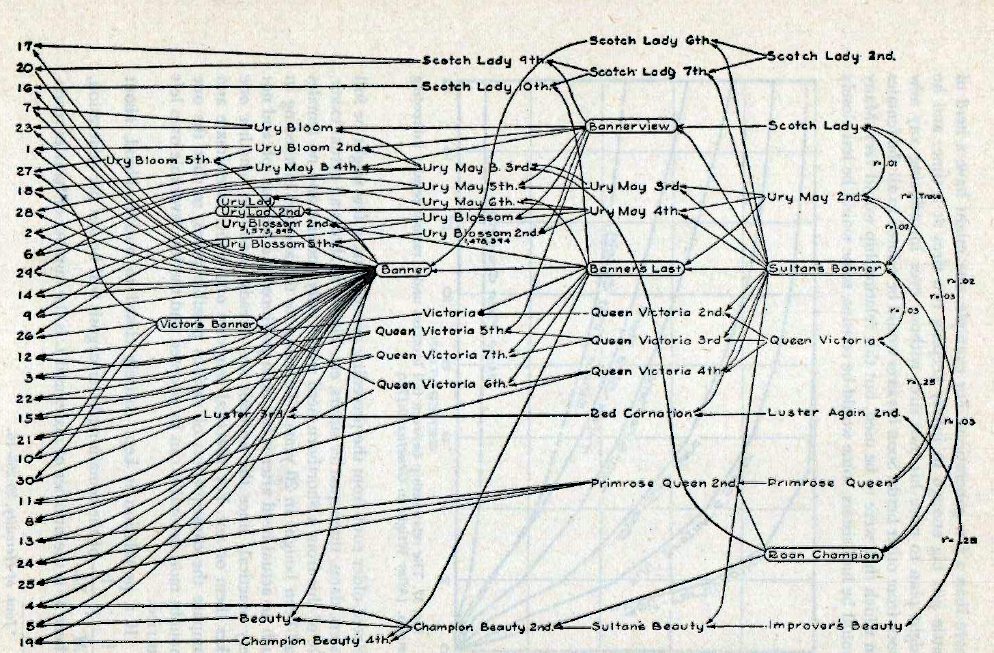
\includegraphics[width=\textwidth]{Figure_38.png}
    \caption{Pedigree of a Shorthorn herd in which no animal had been introduced for 17 years and but 
    		 one in 20 years. The herd was built largely around Sultan's Banner with some secondary 
    		 linebreeding to his sons, Bannerview and Banner's Last and quite a bit of
			 secondary linebreeding to his double grandson, Banner. (From \textit{Jour. of Heredity}, 
			 25:208.)}
    \label{fig:Lush_Figure_38}
\end{figure}

By this formula we can calculate where purebred systems with rigidly
closed herdbooks are drifting, so far as concerns any inbreeding
which is inevitable because the members of a pure breed are becoming
more closely related to each other. Even in a small breed with 200 sires
and 2,000 dams used per generation, the formula shows only .069 per
cent of the heterozygosis lost per animal generation. In other words it
would take about 15 animal generations to lose 1 per cent of the remaining
heterozygosis in such a small breed. There need be no fear that a
closed herdbook will automatically lead to dangerously high inbreeding,
even though the herdbook remains closed and the breed remains
moderately small for centuries. However, show rings, advertising, and
other sales efforts make some males more popular than others. These
males have many sons and grandsons which go to head other registered
herds. Less popular sires have no sons which see service in purebred
herds and perhaps few daughters and no grandsons. This has the effect
of making \textit{M }in the formula much smaller than the actual number of
males which have registered daughters in each generation. In several
pure breeds so far studied, the decrease in heterozygosis per generation
on account of the inbreeding practiced is not very far from 0.4 to 0.6 per
cent. Even so, only about 10 to 12 per cent of the present amount of
heterozygosis would disappear in another century of pure breeding like
that of the last 30 years. An occasional undetected fraudulent registration
of a grade would further reduce this rate.
\index{Heterozygosis|)}
\index{Inbreeding!in isolated populations|)}

\section*{COMPLETE FORMULA FOR THE MEASUREMENT OF RELATIONSHIP}
\index{Relationship!measurement of|(}

The measures of relationship can now be corrected for the effects of
inbreeding. The complete formula for the coefficient of relationship
between animals \textit{X} and \textit{Y} is:

\[R_{XY} = \frac{\Sigma[{1/2}^n(1 + F_A)]}{\sqrt{1 + F_X}\sqrt{1 + F_Y}} \]

\noindent
where \textit{n} is the total number of Mendelian segregations in the path of
descent through which \textit{X} and \textit{Y} are related. This differs from the
approximate formula used in the last chapter only by having terms for
the inbreeding of \textit{X} and \textit{Y} and of their common ancestor. The $(1 + F_A)$
in the numerator allows for the fact that an inbred ancestor (\textit{A}) is
homozygous for more pairs of genes than a non-inbred one. Its use is
illustrated in Figure~\ref{fig:Lush_Figure_35} where the inbreeding of I adds to the relationship
betwen itself and III, or the inbreeding of \textit{M} increases the relationship
between \textit{K} and \textit{L}. The terms in the denominator are to correct for
the fact that inbreeding makes the population more variable, the inbred
lines tending to drift apart from each other. Relationship is a fraction
which has for its numerator the number of genes in which the two
related animals are probably alike but which would be unlike in two
random animals from the base population, and for its denominator the
average number of genes in which two animals probably would be
unlike if they were unrelated but descended from the base population
by the same kind of breeding system as the two actually are. The
denominator grows larger with their inbreeding because the inbreeding
tends to decrease the proportion of heterozygosis and to throw the
population toward the two homozygous extremes in each pair. In a
highly inbred population two unrelated individuals (necessarily from
different inbred lines if they are unrelated) have a considerably larger
chance of being \textit{AA} and \textit{aa} than if they were from a non-inbred population,
because in the inbred population there are more \textit{AA} and \textit{aa} and
fewer \textit{Aa} individuals present. This increase in the denominator naturally
lowers the relationship unless there is a corresponding or greater
increase in the numerator. Such an increase in the numerator can and
usually does occur if the two animals are members of the same inbred
line but not if they belong to lines which have separated and no longer
interbreed with each other.

The complete formula for relationship between an animal and its
ancestor where there is no collateral relationship may be written

\[ R_{XA} = \Sigma[{1/2}^n]\sqrt{\frac{1 + F_A}{1 + F_X}} = \text{``Percentage of blood'' times }\sqrt{\frac{1 + F_A}{1 + F_X}} \]

\noindent
If \textit{A} and \textit{X} are equally inbred, the term under the square root sign
equals 1.0 and the percentage of blood is exactly equal to the coefficient
of relationship. If the ancestor is more highly inbred, the figure for percentage
of blood is not quite large enough. This is because there will be
more than the average number of cases in which the ancestor is homozygous
and therefore both its genes in that pair will be like the one its
descendant receives from it. If the descendant is more highly inbred, the
figure for percentage of blood is a little too large. This is because there
will be cases in which the descendant is homozygous for a gene heterozygous
in the ancestor. In such gene pairs the descendant gets 100 per
cent of its genes from that ancestor and yet is not 100 per cent like the
ancestor. For an example we may return to the pedigree of \textit{X}
(page \pageref{fig:Lush_Figure_Page-273})
which was a double grandson of \textit{A}. In one-fourth of the cases for any
one pair of genes, \textit{X} gets both its genes from the grandams and none
from \textit{A}; in one-half the cases, \textit{X} gets one gene of the pair from \textit{A} and
the other from a grandam; in the remaining one-fourth of the cases, \textit{X}
gets both genes from \textit{A}. On the average, therefore, \textit{X} gets 50 per cent of
its inheritance from \textit{A}, just as the percentage of blood figure shows.
However, in the one-eighth of the cases when \textit{X} is \textit{rr} or \textit{RR}, it will get
both genes from \textit{A} but yet will not be exactly like him, because he was
\textit{Rr}. The corrections in the denominator thus keep the relationship
coefficient a measure of probable genetic likeness and not merely a
measure of source of the genes, as is percentage of blood. Not often is
the difference in the inbreeding of \textit{A} and \textit{X} large enough to be important.
A much more serious general defect of percentage of blood as a
measure of relationship is that it does not include collateral relation ship
and that collateral relationship cannot readily be measured by any
way of manipulating percentage of common blood.

In the pedigrees ordinarily encountered in actual animal breeding,
the denominator of the relationship coefficient does not get very much
larger than 1.0. Neglecting it altogether is not apt to lead to a serious
mistake. However, it must be included if the formula is to be entirely
correct. It is not often worthwhile to carry the computation of either
\textit{R} or \textit{F} for individual animals farther than to the nearest 1 per cent.
Often the nearest 5 per cent is close enough. The sampling variations
inherent in Mendelism prevent one from being sure that the computed
coefficient describes with extreme accuracy the actual situation in individual
cases, even if one could make practical use of small differences
in these coefficients.

The similarity between the formula for inbreeding and the complete
formula for relationship shows how it is that an individual's
inbreeding depends upon the relationship between its sire and its dam.
The equations connecting the two, where \textit{S} represents the sire, \textit{D} the
dam, and \textit{O} the offspring, are:

\[ F_O = \frac{R_{SD}}{2} \times \sqrt{(1 + F_S)(1 + F_D)}, \text{and} \frac{R_{SD}}{2} = \frac{2F_O}{\sqrt{(1 + F_S)(1 + F_D)}} \]

\noindent
Unless the sire and dam are highly inbred, the term under the square
root sign will not differ much from 1.0; and it will be approximately
correct to say that the inbreeding of the offspring is one-half of the relationship
between its parents. This rule is useful when estimating the
amount of inbreeding danger in a mating before that mating is made.
\index{Relationship!measurement of|)}

\section*{OTHER PROCESSES WHICH CAN AFFECT HOMOZYGOSIS}

The inbreeding coefficient expresses probable changes in homozygosis
based on no other assumptions than that inheritance is Mendelian
and is equal from the two parents. It neglects sex-linkage\index{Sex linkage} and the small
changes in homozygosis which may be made by mutation and selection
and by assortive mating which is not inbreeding.

So far as concerns sex-linked genes, the inbreeding coefficient for the
pedigree of a heterogametic animal has no meaning. The heterogametic
parent behaves as if it were entirely homozygous for sex-linked
genes in transmitting to its homogametic offspring, and transmits no
sex-linked genes at all to its heterogametic offspring. Referring for convenience
to the female as the homogametic sex (as is correct for the
mammals but not for the birds and a few other animals), the inbreeding
computed for a female's pedigree is not true for her sex-linked genes
wherever the line of descent is from sire to son. On the other hand,
wherever the line of descent is from sire to daughter, the homozygosity
of females for sex-linked genes will be higher than the coefficient indicates.
These two effects tend partly to cancel each other so that the
inbreeding coefficient will generally measure the extra homozygosity of
females, even for sex-linked genes. There will be cases where the coefficient
will be systematically in error for the sex-linked genes; e.g., a
double granddaughter of a male would not tend to have her sex-linked
genes any more homozygous than if her parents had been unrelated,
while a double granddaughter of a female would have her sex-linked
genes 25 per cent less heterozygous instead of the expected 12½ per
cent.\footnote{A more detailed explanation of the consequences of inbreeding on
the distribution of sex-linked genes was presented by Wright in 1955.
\textit{Proc. Nat. Acad. Sci.}, 19:411--20.}

Mutation\index{Mutations} is so rare an event that its neglect in the formula introduces
no error of importance in practical breeding, although mutation
needs to be included in evolutionary considerations where the time
involved extends over an enormous number of generations. The formulas
for including it are rather intricate.\footnote{\textit{Genetics}, 16:116--37.}

\index{Selection!and homozygosis}
Selection affects homozygosis only incidentally through changing \textit{q}
and thereby the value of $2q (1 - q)$. Selection will usually require many
generations to make large changes in \textit{q}, except in those cases where
intense selection is directed at a characteristic the main variations of
which are highly hereditary and are determined by a very few genes.
The effects of :;election on homozygosis certainly need to be considered
in connection with problems of evolution, but in general they are
probably too small to make inbreeding coefficients much in error as
measures of the change in homozygosis which has occurred within the
last four to six generations. Assortive mating (as will be explained in
chapters 27 and 28) has almost no effect on homozygosis except when
(l) the assortive mating is almost perfect, (2) the characteristics concerned
are highly hereditary, and (3) the number of genes producing the
observed variation is small. Very rarely would all these conditions be
met in actual practice.

\section*{PRACTICAL USES OF INBREEDING}
\index{Inbreeding!practical uses of|(}

Most breeders inbreed only when they must to attain some other
object, such as linebreeding or forming and preserving family distinctness.
The commonest reason for inbreeding is that a breeder must do
some of it if he is to keep his animals closely related to individual animals
he admires. Relationship between two animals cannot go higher
than 50 per cent unless there has been some inbreeding. If a breeder
continually uses unrelated sires, the relationship of each succeeding
generation to the animals he has had in his herd will be halved. In a
short time his animals will be very little related to the best ones of two
or more generations ago. If he still has a good herd, that will be because
he has been successful in selecting his subsequent sires. If, instead of
using unrelated sires each generation, he uses sires closely related to the
best animals he has had, then he may keep the future generations as
closely related to those good ancestors as his present animals are. But,
since both sires and dams of his stock are related to these good animals,
he will be practicing some inbreeding. This is the essence of ``linebreeding,''
which is the subject of Chapter 23. In this practice most breeders
regard inbreeding as a necessary evil which must be endured if they are
to keep their herd closely related to some noted animal, but which
should be kept as low as can be done and still accomplish the linebreeding
program.

If the homozygous recessives can all be discarded, inbreeding can be
a powerful help to selection against rare recessives. There may be so
many recessives in the stock that the inbreeding will bring them to light
in more animals than the breeder can afford to discard, or he may not
recognize some of those with the less conspicuous effects in time to discard
them before they become fixed on his whole herd. This is what
breeders have in mind if they say that their breed is not yet perfect
enough to make even linebreeding wise as a general policy. The price
which must be paid for using inbreeding thus to improve the breed is
the occurrence at first of a larger proportion of undesirable individuals.
That price may be so high that the individual breeder will not find it
economically possible for him to practice extremely close inbreeding as
a steady policy.

Inbreeding may be used to test whether animals are good enough to
justify deliberate and long-continued attempts to keep the herd closely
related to them. Inbreeding is the severest test of the hereditary worth
of an individual that can be made. Wriedt goes so far as to recommend
that every dairy bull thought worth using in the first place should be
bred as soon as possible to enough of his daughters to insure that there
will be at least 15 or 20 of his daughters out of his own daughters to
prove his breeding value. For several reasons this proposal seems too
extreme for general adoption. However, it does rest on the truth that
inbreeding is the severest and quickest test to find whether an animal
has any undesired genes.

Inbreeding can be used to promote homozygosity. Homozygosity has
little commercial value in the sale ring as yet. Hence it seems unlikely
that many breeders could afford to inbreed intensely just for this object.
Nevertheless, homozygosity is the most important element in prepotency,
and the building of this into his herd is worth some effort by the
breeder, provided he can maintain or improve the average phenotypic
merit at the same time.
\index{Homozygosis|)}

A breeder often practices inbreeding merely for economy. This is
an unwise policy whenever the animals are of only average merit. He
could then expect only offspring of average merit, even if there were no
inbreeding. With the added probability of some phenotypic degeneration
from inbreeding, he can expect the offspring to be below the average
merit of their breed as individuals, although not necessarily below
the breed average in their merit as breeding animals. When the animal
to which the inbreeding is being directed is of superior merit, this reason
of economy lends additional weight to the argument for inbreeding.

One of the important general reasons for practicing inbreeding is
that it tends to form distinct families within the breed and thus permits
more selection between families than would be possible under random
breeding. (This will be discussed in more detail in Chapter 24). Selection
between families can be much more accurate than selection
between individuals, especially for characteristics which are only slightly
hereditary; but the families must be rather distinct from each other if
that is to be the case. The family averages of non-inbred families do not
deviate from each other as much as individual genotypes do.

The producer of market animals has little reason to practice
inbreeding. His market will not pay him any extra for prepotency.
Improvements he may make in the average merit of his own herd by
using inbreeding along with selection will be about halved next time he
buys an unrelated sire from some other source, as most commercial producers
do. Economy can be a valid reason with him, especially when he
thinks the sire he has is better than the next one is likely to be. Partly
offsetting this superiority of his present sire is the probability that
some harmful results of inbreeding will occur in his herd.)
\noclub
\index{Inbreeding!practical uses of|)}

\section*{THE DANGERS OF INBREEDING}
\index{Inbreeding!dangers of|(}

Inbreeding makes desirable and undesirable genes homozygous
impartially. If the rate of this is too rapid, every individual produced
will be homozygous for some undesired genes as well as for some desired
ones\index{Variation!increased by inbreeding}. If the inbreeding is too mild, many generations will be needed to
accomplish much with it. The problem of the best rate at which to
inbreed is one of keeping the inbreeding mild enough that the man in
charge can avoid fixing the genes with undesirable effects and can fix as
many as possible of the genes which have desirable effects. How mild or
how intense such inbreeding can be depends upon several things, the
most important of which are the skill of the man doing the selecting,
the abundance of undesired genes in the stock with which he begins, the
amount of linkage between desired and undesired genes in the initial
stock, the amount of epistasis, dominance, or environmental effects
which may deceive the breeder when he makes his selections, and
whether he is breeding a group all by himself. If other men are breeding
closely related lines, he can correct his mistakes by mild outcrosses
to some of their herds without having to use totally unrelated animals.

Fragmentary evidence of various kinds indicates that inbreeding
rates as high as 6 per cent per generation\footnote{As, for example,
in a two-sire herd where no outside blood is introduced.} under favorable
circumstances may be pursued for many generations without noticeably
harmful consequences. It is unlikely that inbreeding rates as high as 3 or 4
per cent can go on forever without harm, but certainly they can be continued
for many generations. Many breeders when in possession of
unusually good animals have had favorable results from mating half
brother to sister or grandsire to granddaughters, but not many have
continued to do that for more than two or three successive generations.
Occasional matings of parent and offspring or, more rarely, full brother
and sister have turned out well; but general experience is that those
should be risked only when the stock is unusually good.

Among human beings inbreeding as intense as the marriage of first
cousins has enough probability of undesired consequences that in some
places it is forbidden by law or religious rule.\footnote{See page 52
of \textit{Time} for August 19, 1940, for a list of marriages forbidden by the
Church of England in 1560. In 1945 prohibitions against ten of these categories of
in-law marriages were removed. This was the first change in those rules in nearly
four hundred years.} Inbreeding more intense
than that is regarded as ``incest'' in nearly all human societies although
there have been some exceptions, as among the Pharaohs in ancient
Egypt. No doubt the biological principles are the same in man as in
other organisms, although the abundance of undesired recessives may
be higher or lower. An extremely important practical difference is that
in farm animals, if inbreeding brings to light a few more defectives
than would occur without it, they may be culled with only the small
economic loss that their defectiveness entails; whereas in most civilized
communities of man the codes of ethics and morals do not permit such
drastic action with defective human beings. The care and support of
each one too defective to take care of itself is a serious burden, whether
it is kept in a private home or in a special institution. Rigid prohibitions
of marriages of a certain degree, such as between first cousins, do
not allow for the fact that such marriages may be desirable when the
common ancestry is of unusual merit. Prohibiting the marriage of relatives
does not improve the average heredity of a population. Neither
inbreeding nor outbreeding makes the undesired genes systematically
either rarer or more abundant, but inbreeding does bring them together
so that more of them can show their effects and be culled-if selection
is being practiced. Perhaps the general experience of man over centuries
may be considered as indicating that around 6 per cent is in general
the ``stop, look, and listen'' level of danger from inbreeding? If the
common ancestry is of sound stock, the children of such marriages may
be above average in merit. If the common ancestry has any serious
defect, even a rare one, the probability of that defect reappearing in the
children who have a chance to inherit it from both sides is much higher
than if their parents were unrelated. The rarer the defect in the general
population, the more extreme is this difference.

The inbreeding coefficient may be used to estimate the danger
involved in any particular mating, if one considers also the merit of the
ancestors from which the inbreeding comes. Inbreeding of 25 per cent
coming from an outstanding ancestor might be safer than inbreeding of
10 per cent coming from a mediocre ancestor. Setting a definite percentage
of inbreeding as the point where danger begins is much like
setting a certain speed in automobile driving as the speed beyond which
danger begins. In the case of the automobile much depends upon the
condition of the highway, the field of vision, the mechanical condition
of the car and the skill of the driver. Similarly with inbreeding, much
depends upon the clearness of the goal, the accuracy of the tests and
measures of merit, the initial scarcity of undesirable genes in the stock,
the amount of culling which the reproductive rates permit, and the
breeder's ability to recognize and discard genes which are on the verge
of becoming fixed in his stock.
\index{Inbreeding!dangers of|)}

\section*{POSSIBILITIES OF PRODUCING INBRED LINES FOR COMMERCIAL CROSSING}

Corn breeders have made a distinct success of producing inbred
lines by self-fertilization and then crossing those lines which produce
the most desirable crosses. The crossbred seed is sold for the production
of commercial corn. Although the fundamental principles are the
same, there are several differences in their application which make the
success of such a breeding system appear less likely for animals than for
plants, although modified systems based on the same principles may
perhaps prove successful. In the first place, the closest possible inbreeding
in animals is less than half as intense as self-fertilization. It would
take many more generations with animals to reach the same degree of
homozygosity. In the second place, the fertility of animals is lower than
that of plants, so that not nearly as large a percentage of the individuals
produced in each generation could be discarded. In the third place,
the interval between generations in farm animals is longer than with
annual plants; and the amount of time required to reach an equal
degree of inbreeding would be longer for that reason also. In the fourth
place, the individual animal is worth more money than the individual
plant. Culling the undesired individuals which appear during the
inbreeding will be more expensive than the same process applied to
plants. In the fifth place, and partially offsetting these others, is the fact
that the merits and faults of individual animals are usually better
known than is the case with individual plants. Therefore, the individual
selection which accompanies the inbreeding would be more
accurate in animals. In the sixth place, the lower fertility of animals
would make it economically difficult to sell the commercial producer as
many as he would need of the crossbred stock from two successfully
inbred lines, if such should ever be produced, or to sell him inbred
females of one line and inbred males of another line so that he could
make his own crosses. Poultry and swine seem more nearly suited to the
economics of that than the other farm animals.

For those reasons commercial animal breeding will never practice
such intense inbreeding alternating with such extreme outbreeding as
is already practiced in corn breeding. On the other hand, a mild form
of this is already happening in the crossbreeding which is practiced for
producing commercial meat animals and in the practice, among breeders
of purebred stock, of making outcrosses between distinctly unrelated
lines within a breed, hoping thereby to produce excellent individuals.
Perhaps it may be commercially possible to produce highly inbred sires
to be used on practically random-bred high grade or purebred females.
At present stockmen set so much store by individuality in their sires
that few of them would use inbred sires unless these were also good
individuals, but that would change quickly if it were demonstrated
clearly that such use would be profitable.

\section*{EXPERIMENTS ON INBREEDING}

Thorough and extensive experiments on inbreeding have been
more numerous with plants than with animals. Many of the facts
about inbreeding were discovered in experiments with corn. More come
from the contrasting behavior of naturally self-fertilized and naturally
cross-fertilized plants when those are experimentally inbred or are used
in various crosses. Conspicuous examples of plants which in nature
have a high percentage of self-fertilization include wheat, cotton, sorghum
and oats. Corn and beets are examples of naturally cross-fertilized
species on which extensive experiments with inbreeding have led to the
production of inbred lines and the sale of crossbred seed on a commercially
important scale. Strawberries and raspberries show much the
same results as corn and beets, but the application is different because
vegetative multiplication of the former is practical.

Among animals, laboratory experiments have been extensive on the
inbreeding of rats, mice, and guinea pigs. Dr. King inbred white rats
full brother and sister for more than 70 generations without finding
degeneration. Mice have been inbred full brother and sister in many
experiments. In at least one case this has been carried further than the
55th generation.\footnote{\textit{Jour. of Heredity}, 27:21--24, 1936.}
In the United States Department of Agriculture
experiments on inbreeding guinea pigs, some lines have been inbred
brother by sister for more than 30 generations. There have been several
short experiments on inbreeding chickens and swine at a number of
experiment stations. In 1945 the 38 lines being studied in the Regional
Swine Breeding Laboratory ranged from about 10 to 70 per cent in
inbreeding. Twelve of them were already inbred more intensely than
three generations of full brother by sister and ten more were nearly that
far along. Inbreeding experiments with poultry at the Iowa Station
have reached a more intense stage than that of nine generations of full
brother by sister mating, although the breeding system actually used
was not that regular.

In farm animals other than chickens and swine, the small number of
full sibs and the variations in the sex ratio prevent the long-continued
use of such regular inbreeding systems as full brother by sister. Even in
chickens and swine these are serious difficulties and reduce tremendously
the amount of selection which can be practiced while the inbreeding
is being done. For the other farm animals the most intense inbreeding
plan which can be followed long is the use of a sire on his daughters as
long as he lives, he to be followed by one of his inbred sons, which in
turn would be followed by one of his inbred sons, and so on. There
would be a few full brother by sister matings and some of the females
would live longer than others, some, perhaps, even outliving two generations
of sires. Hence such a system of inbreeding would be far from
regular, and there would be comparatively few pedigrees which were
exactly alike in the kinds of inbreeding they showed over a period of
three or four generations. Before an inbreeding coefficient was devised
for measuring the intensity of the irregular inbreeding shown in these
many kinds of pedigrees, it was natural that experimenters should think
that inbreeding experiments of that kind could not be interpreted in
any unmistakable way and therefore would not return scientific information
worth the money and effort they would cost. Now that Wright's
coefficient of inbreeding, which was first proposed in 1922, largely
removes this objection, it is probable that more experimental study will
be made of irregular systems of inbreeding.

Some of what we know about the results of inbreeding in animals
comes from the scattered and irregularly reported experience of breed ers.
It is difficult to be at all sure that such evidence is a typical sample
of the results of inbreeding. There is the question of whether the animals
inbred were typical of purebred animals in general. There is also
the question of whether one hears of the typical results of such cases or
only of the exceptional results. Any bad result which does appear is apt
to be blamed on the inbreeding in spite of the fact that equally bad
results sometimes occur when no inbreeding is practiced. There is
usually an absence of adequate control; that is, of non-inbred animals
kept under the same conditions. However, the results agree in general
with those expected on theoretical grounds and with those actually
obtained in laboratory experiments. The usual consequences of
inbreeding in breeders' experiences is a degeneration which, however,
is slight and irregular, affecting some characteristics in one animal and
other characteristics in another and not affecting some individual animals
at all. Even in Bakewell's time it was known and stressed that
inbred animals are more apt to be prepotent and effective when used in
outcrosses than are animals of equal individuality but not inbred.

The breeders who have practiced intense inbreeding for a long time
have nearly always encountered enough degeneration that a cross with
unrelated animals produced beneficial results. So universal has this
experience been that breeders are rather generally convinced of the
necessity of introducing ``fresh blood'' from time to time to ``rejuvenate''
a strain or herd. It is not always understood that this rejuvenating
effect rarely occurs unless there has been some prior inbreeding. The
explanation of these cases is that the herd becomes homozygous for
undesirable genes which produce such small effects that the breeder
scarcely notices them as they become fixed a few at a time, but instead
just sees a gradual decline in vigor, fertility, size, etc. Since undesirable
genes tend to be recessive, a cross with an animal from an unrelated
herd often appears to remedy these defects at once.

\section*{SUMMARY}

Inbreeding is the mating of animals which have a closer relationship
to each other than the average relationship within the population
concerned. Its measure is relative to some population, just as the measure
of relationship is. Pure breeding is inbreeding relative to the whole
species, but not many purebred animals are closely inbred relative to
their breed.

The primary effect of inbreeding is to make more pairs of genes
hortiozygous and to lower the percentage of heterozygosis correspondingly.
Because this uncovers many recessive genes which would otherwise
remain concealed by their dominant alleles, and because recessives
generally have less desirable effects than dominants do, there is usually
some degeneration in average individual merit when inbreeding is
practiced.

Inbreeding does not of itself change gene frequency but does permit
it to drift rapidly at random in each subgroup of the population.
Inbreeding is the most powerful tool the breeder has for establishing
uniform families or strains which are distinct from each other. This
it does by permitting gene frequencies to drift in different ways in different
subgroups, by making the parents more homozygous, and by
providing more and more ways in which members of the same family
are likely to inherit the same genes because their parents are related to
each other.

Some inbreeding is almost essential if selection is to have much success
in those cases where a highly desirable effect is produced by a combination
of genes which individually have undesirable effects; that is,
for getting a population out of some of the lower ``peaks of desirability''
shown in Figures~\ref{fig:Lush_Figure_20} and \ref{fig:Lush_Figure_21} and
into higher nearby peaks.

The coefficient of inbreeding measures the percentage of genes
which were heterozygous in the basic population but have probably
become homozygous because of the inbreeding. It is subject to the sampling
errors of Mendelian inheritance and hence means almost nothing
for one pair of genes in one individual, but its sampling error may be
small when it is applied to the average percentage of heterozygosis of
one pair of genes in a whole population or to the average heterozygosis
of the entire group of genes in one individual.

Among the more important reasons for practicing inbreeding are:
(1) It is necessary if relationship to a desirable ancestor is to be kept
high; (2) it helps uncover rare recessives so that they may be culled from
the breed; (3) it forms uniform and distinct families so that interfamily
selection may be possible in a more effective way than if inbreeding
were not practiced; (4) it increases prepotency; and (5) it is sometimes
economical, especially if the present sire is of such high merit that it
will be difficult to find as good a one for a successor.

The danger of intense inbreeding is that it will make undesired
genes homozygous at so rapid a rate that it will be impossible to discard
all individuals homozygous for them. Some of the undesired genes will
therefore become ``fixed'' in the whole herd. The lowered sale value of
the defectives uncovered by the inbreeding will cause some loss. From
the standpoint of breed improvement, that loss is balanced by the
increased prepotency of those which are not defective; but the man who
is breeding animals for the commercial market will not receive that
compensation.

It seems reasonably certain that more opportunities for breed progress
are lost by not inbreeding when inbreeding would be advisable
than are lost by too much inbreeding. When inbreeding is too intense,
the individual breeder may lose by that; but the progress of the breed
is not apt to suffer. The best of the inbred animals are likely to give
good results in outcrosses.

\section*{REFERENCES}

The general subject of inbreeding was treated comprehensively in
the following book, which, even a quarter of a century later, is obsolete
in little except its treatment of the measurement of inbreeding
intensity:

\begin{hangparas}{0.5in}{1}%
East, E. M., and Jones, D. F. 1919. Inbreeding and outbreeding. Philadelphia The
J. B. Lippincott Co. 285 pp.
\end{hangparas}

For explanation of the Mendelian basis of inbreeding and of what
happens when various rates of inbreeding, mutation, and selection are
balanced against each other, see:

\begin{hangparas}{0.5in}{1}%
Wright, Sewall. 1921. Systems of mating. Genetics, 6:111--78.

---. 1922. Coefficients of inbreeding and relationship. Amer. Nat., 56:330--38.

---. 1923. Mendelian analysis of the pure breeds o livestock. I. The measurement
of inbreeding and relationship. Jour. of Heredity, 14:339--48.

---. 1923. Mendelian analysis of pure breeds of livestock. II. The Duchess
family of Shorthorns as bred by Thomas Bates. Jour. of Heredity, 14:405--22.

---. 1931. Evolution in Mendelian populations. Genetics, 16:97--159.

---. 1940. Breeding structure of populations in relation to speciation. Amer.
Nat., 74:232--48.
\end{hangparas}

For reports of actual experiments on inbreeding animals, see:

\begin{hangparas}{0.5in}{1}%
Castle, W. E. 1930. Genetics and Eugenics, pp. 286--304. Cambridge: Harvard University
Press.

Hodgson, R. E. 1935. An eight-generation experiment in inbreeding swine. Jour.
Heredity, 26:209--17.

Hughes, E. H. 1933. Inbreeding Berkshire swine. Jour. Heredity, 24:199--203.

King, Helen Dean. 1918 and 1919. Studies of inbreeding. Jour. of Exp. Zoology,
26:1--54, 26:335--78, 27:1--36, and 29:71--112.

Strong, Leonell C. 1936. The establishment of the ``A'' strain of inbred mice. Jour.
Heredity, 27:21--24.

USDA Yearbook for 1936.

Waters, N. F., and Lambert, W. V. 1936. Inbreeding in the White Leghorn fowl.
Iowa Agr. Exp. Sta., Res. Bul. 202.

Willham, 0. S., and Craft, W. A. 1939. An experimental study of inbreeding and
outbreeding in swine. Okla. Agr. Exp. Sta., Tech. Bul. 7.

Woodward, T. E., and Graves, R. R. 1933. Some results of inbreeding grade Guernsey
and grade Holstein-Friesian cattle. USDA, Tech. Bul. 339.

Wright, Sewall. 1922. The effects of inbreeding and crossbreeding on guinea pigs.
I. Decline in vigor. II. Differentiation among inbred families. USDA,
Department Bul. 1090. III. Crosses between highly inbred families, USDA,
Department Bul. 1121.

---, and Lewis, Paul A. 1921. Factors in the resistance of guinea pigs to tuberculosis,
with special regard to inbreeding and heredity. Amer. Nat., 55:20--50.
\end{hangparas}

For brief statements of breeders' experience with regard to inbreeding,
see:

\begin{hangparas}{0.5in}{1}%
Mumford, F. B. 1921. Breeding farm animals. pp. 217--42.

Wriedt , Christian. 1930. Heredity in livestock. pp. 68--115.
\end{hangparas}

For studies of the amount and kind of inbreeding which has
occurred in various breeds of livestock, see:

\begin{hangparas}{0.5in}{1}%
Berge, S. 1930. Inbreeding in Telemark cattle. (Translated title). Nordisk Jordbrugsforskning
204--16.

Brockelbank, E. E., and Winters, L. M. 1931. A study of the methods of breeding the
best Shorthorns. Jour. Heredity, 22:245--49.

Calder, A. 1927. The role of inbreeding in the development of the Clydesdale breed
of horses. Proc. Royal Soc. of Edinburgh, 47, Part 2, No. 8, pp. 118--40.

Carter, Robert C. 1940. A genetic history of Hampshire sheep. Jour. Heredity,
31:89--93.

Dickson, W. F., and Lush, Jay L. 1933. Inbreeding and the genetic history of the
Rambouillet sheep in America. Jour. Heredity, 24:19--33.

Fletcher, J. Lane. 1945. A genetic analysis of the American Quarter Horse. Jour.
Heredity, 36:316--352.

---. 1946. A study of the first fifty years of Tennessee Walking Horse breeding.
Jour. Heredity, 37:369--373.

Fowler, A. B. 1932. The Ayrshire breed: A genetic study. Jour. of Dy. Res., 4:11--27.

L\"ortscher, H. 1945. Inbreeding and relationship among the Jura horses today.
(translated title). Landw. Jahrb. d. Schweiz, pp. 1--16.

Lush, Jay L. 1946. Chance as a cause of changes in gene frequency within pure
breeds of livestock. Amer. Nat. 80:318-342.

---, and Anderson, A. L. 1939. A genetic history of Poland-China swine.
Jour. Heredity, 30:149--56 and 219--24.

---; Holbert, J. C.; and Willham, 0. S. 1936. Genetic history of the Holstein-
Friesian cattle in the United States. Jour. Heredity, 27:61--71.

McPhee, Hugh C., and Wright, Sewall. 1925. Mendelian analysis of the pure breeds
of livestock. III. The Shorthorns. Jour. Heredity, 16:205--15.

---. 1926. Mendelian analysis of the pure breeds of livestock. IV. The British
Dairy Shorthorns. Jour. Heredity, 17:397--401.

Rottensten, Knud. 1937. Inbreeding in Danish Landrace swine. (Translated title).
Nordisk Jordbrugsforsknmg, Hefte 3--4A, pp. 94--114.

Sciuchetti, A. 1935. Ein Beitrag zur genetischen Analyse der schweizerischen Braunviehrasse.
Julius Klaus-Stiftung f. Vererb. Sozialanthr. u. Rassenh., 10:85--99.

Smith, A. D. B. 1926. Inbreeding in cattle and horses. Eugenics Review, 18:189--204.

Steele, Dewey. 1944. A genetic analysis of recent Thoroughbreds, Standardbreds, and
American Saddle Horses. Kentucky Agr. Exp. Sta., Bul. 462.

Stonaker, H. H. 1943. The breeding structure of the Aberdeen-Angus breed. Jour.
Heredity 34:322--28.

Willham, 0. S. 1937. A genetic history of Hereford cattle in the United States.
Jour. Heredity, 28:283--94.

Yoder, Dorsa M., and Lush, Jay L. 1937. A genetic history of the Brown Swiss cattle
in the United States. Jour. Heredity, 28:154--160.
\end{hangparas}
\index{Inbreeding|)}